\documentclass[hyperref={pdfpagemode=FullScreen,colorlinks=true},xcolor=pst,dvips]{beamer}\usepackage[french]{babel}
\usepackage[T1]{fontenc}
\usepackage[utf8]{inputenc}
\usepackage{lmodern}
\usepackage{microtype}
\usepackage{hyperref}
\usepackage{tabulary}
\usepackage{framed}
%\usepackage{fancyhdr}
\usepackage{amsmath}
\usepackage{bbm}
\usepackage{pstricks}
\usepackage{ulem}
		
\usetheme{Madrid}
\useinnertheme{rectangles}

\title[]{\rule{\linewidth}{1pt}
		\large Recherche de filtres de Bloom similaires \\
		\large Application à la recherche par mots clés basée sur une DHT\\
		\rule{\linewidth}{1pt}
}
\author[NDOMBI TSHISUNGU \& DOAN]{\textbf{NDOMBI TSHISUNGU} Christian \& \textbf{DOAN} Cao Sang \\
			Encadrant: M. \textbf{MAKPANGOU} Mesaac, Regal}
\institute{UPMC}
\date{2 Mai 2015}

\begin{document}

	\begin{frame}
		\titlepage
	\end{frame}
	
	\begin{frame}
		\frametitle{Table de contents}
		\tableofcontents
	\end{frame}
	
	\section{Présentation}
	\subsection{Problème classique}
	\begin{frame}
		\frametitle{Présentation}
		\framesubtitle{Problème classique}
		\begin{itemize}
			\item volume de données de plus en plus importants
			\item accès à l'information $\rightarrow$ \textbf{efficacité}(Temps et coût)
		\end{itemize}
		\begin{figure}[!htbp]
			
\includegraphics[width=3cm]{image1.eps}
			
\includegraphics[width=6cm]{image2.eps}
			
\includegraphics[width=3cm]{image.eps}
		\end{figure}		
	\end{frame}
	
	\subsection{Nos solutions}
	\begin{frame}
		\frametitle{Présentation}
		\framesubtitle{Nos solutions}	
		\begin{itemize}
			\item Approche: Filtre de Bloom
			\item \sout{Méthode d'accès FreeCore: Indexation(Listes inversées)}
			\item Méthode d'accès: Indexation(Vecteur d'approximation)
		\end{itemize}
	\end{frame}

	\section{Filtre de Bloom}
	\begin{frame}
		\frametitle{Filtre de Bloom}
		\begin{table}[!h]
		\centering		
		\begin{tabular}{|l|*{14}{c|}r|}
		\multicolumn{1}{c}{{\scriptsize 15}} &\multicolumn{1}{c}{}&\multicolumn{1}{c}{}&\multicolumn{1}{c}{}&\multicolumn{1}{c}{}&\multicolumn{1}{c}{}&\multicolumn{1}{c}{}&\multicolumn{1}{c}{}&\multicolumn{1}{c}{}&\multicolumn{1}{c}{}&\multicolumn{1}{c}{}&\multicolumn{1}{c}{}&\multicolumn{1}{c}{}&\multicolumn{1}{c}{}&\multicolumn{1}{c}{}&\multicolumn{1}{c}{{\scriptsize 0}}\\
		\hline
			1 & 0 & 0 & 0 & 1 & 1 & 0 & 1 & 0 & 0 & 0 & 0 & 1 & 0 & 0 & 0 \\
		\hline
		\end{tabular}
		\caption{Filtre de Bloom}
	\end{table}	
	\end{frame}	
	
	\begin{frame}[shrink]
		\frametitle{Filtre de Bloom}
		\begin{figure}[!htbp]
			\centering
			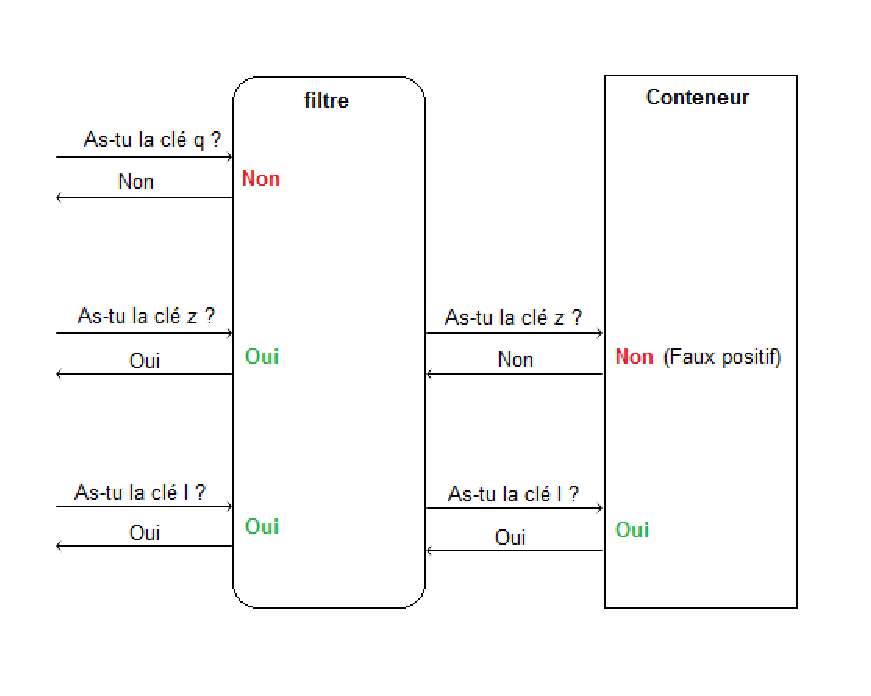
\includegraphics[width=10cm]{ismember.eps}
			\caption{isMember?}
		\end{figure}	
	\end{frame}	
	
	\subsection{Insertion}
	\begin{frame}[shrink]
		\frametitle{Filtre de Bloom}
		\framesubtitle{Insertion dans le filtre de Bloom}
		
		\begin{framed}
		\textbf{IN:} \textit{x} objet à insérer dans le filtre de Bloom \textit{B}\\
		\textbf{FUNCTION:} \textit{insert(x)}\\
		\textbf{OUT:} $\emptyset$
		\noindent\rule{\linewidth}{0.5pt}

		\begin{tabbing}
			\textbf{for} \= $i = 0\ ...\ k - 1$ \textbf{do}\\
					\> $j \leftarrow h_i(x)$\\
					\> \textbf{if} \= $B_j == 0$ \textbf{then}\\
					\> \> $B_j \leftarrow 1$\\
					\> \textbf{end}\\
			\textbf{end}
	    	\end{tabbing}		
	\end{framed}
	\end{frame}
	
	\subsection{Recherche}
	\begin{frame}[shrink]
		\frametitle{Filtre de Bloom}
		\framesubtitle{Recherche dans le filtre de Bloom}
		\begin{framed}
		\textbf{IN:} \emph{x} objet à tester dans le filtre de Bloom \textit{B}\\
		\textbf{FUNCTION:} \textit{ismember(x)}\\
		\textbf{OUT:} $bool$

		\noindent\rule{\linewidth}{0.5pt}

		\begin{tabbing}
			$m \leftarrow true$\\
			$i \leftarrow 0$\\
			\textbf{while} \= $m$ \&\& $i \leq k - 1$ \textbf{do}\\
					\> $j \leftarrow h_i(x)$\\
					\> \textbf{if} \= $B_j == 0$ \textbf{then}\\
					\> \> $m \leftarrow false$\\
					\> \textbf{end}\\
					\> $i \leftarrow i + 1$\\
			\textbf{end}
			\textbf{return} $m$\\
	    	\end{tabbing}		
	\end{framed}
	\end{frame}
	
	\subsection{Exemple}
	\begin{frame}
		\frametitle{Filtre de Bloom}
		\framesubtitle{Exemple}
		\begin{figure}[!htbp]
			\centering
			\includegraphics[width=12cm]{exemple1.eps}
		\end{figure}	
	\end{frame}
	
	\begin{frame}
		\frametitle{Filtre de Bloom}
		\framesubtitle{Approche d'indexation avec le filtre de Bloom}
		\begin{figure}[!htbp]
			\centering
			\includegraphics[width=13cm]{exemple2.eps}
		\end{figure}	
	\end{frame}
	
	\begin{frame}
		\frametitle{Filtre de Bloom}
		\framesubtitle{Approche de vecteur approché}
		\begin{figure}[!htbp]
			\centering
			\includegraphics[width=12cm]{exemple3.eps}
		\end{figure}	
	\end{frame}
	
	\section{Algorithme des fonctions}
	\subsection{CREATE\_FILTER}
	\begin{frame}[shrink]
		\frametitle{Algorithme des fonctions}
		\framesubtitle{CREATE\_FILTER}
		\begin{framed}
		\textbf{IN:} $\sum desc$\\
		\textbf{FUNCTION:} \textit{create\_filter($\sum desc$)}\\
		\textbf{OUT:} \textit{$B^{512}$}\\

		\noindent\rule{\linewidth}{0.5pt}

		\begin{tabbing}
			\textit{init($B^{512}$)}\\
			$x \leftarrow$ FIRST($\sum desc$)\\
			\textbf{while} \= $x \neq \emptyset$ \textbf{do}\\
					\> $i \leftarrow$ SHA\_256(\textit{x})\\
					\> $j \leftarrow i\ mod\ 512$\\
					\> $B^{512}[j]\leftarrow 1$\\
					\> $x \leftarrow$ NEXT($\sum desc$)\\
			\textbf{end}\\
			\textbf{return} $B^{512}$\\
	    	\end{tabbing}		
	\end{framed}
	\end{frame}
	
	\subsection{PUT}
	\begin{frame}[shrink]
		\frametitle{Algorithme des fonctions}
		\framesubtitle{PUT}
		\begin{framed}
		\textbf{IN:} filtre de Bloom de taille 512 bits $B^{512}$\\
		\textbf{FUNCTION:} \textit{put($B^{512}$)}\\
		\textbf{OUT:} \textit{$\emptyset$}\\

		\noindent\rule{\linewidth}{0.5pt}

		\begin{tabbing}
			$i \leftarrow$ MAX\_LEVEL\\
			$vector_i \leftarrow$ CREATE\_VECTOR($B^{512}$, \textit{i})\\
			$x \leftarrow$ FIRST(\textit{VA\_file})\\
			\textbf{while }\= $x \neq \emptyset$ \textbf{do}\\
					\> \textbf{if }\= $vector_i = x$\textbf{ then}\\
					\> \> BREAK\\
					\> \textbf{end}\\
					\> $x \leftarrow$ NEXT(\textit{VA\_file})\\
			\textbf{end}	\\	
	    	\end{tabbing}		
	\end{framed}
	\end{frame}
	
	\begin{frame}[shrink]
		\frametitle{Algorithme des fonctions}
		\framesubtitle{PUT(suite)}
		\begin{framed}
		\begin{tabbing}
			\textbf{if }\= $vector_i \neq x$\textbf{ then}\\
				\> \textit{VA\_file } $\leftarrow$ ADD($vector_i$)\\
			\textbf{end}	\\	

			\textbf{for }\=$i = MAX\_LEVEL\ ...\ 1$ \textbf{do}\\
					\> \textbf{if }\= $i = 1$ \textbf{then}\\
					\> 	\> $vector_i \leftarrow$ CREATE\_VECTOR($B^{512}$, \textit{i})\\
					\>	\> CREATE\_FILE($vector_i,\ B^{512}$)\\
					\> \textbf{else}\\
					\>	\> $vector_i \leftarrow$ CREATE\_VECTOR($B^{512}$, \textit{i})\\
					\>	\> CREATE\_FILE($vector_i$, CREATE\_VECTOR($B^{512}$, \textit{i - 1}))\\
					\> \textbf{end}\\
			\textbf{end}	\\	
			\textbf{return} $\emptyset$\\
		\end{tabbing}
		\end{framed}
	\end{frame}
	
	\subsection{SEARCH}
	\begin{frame}[shrink]
		\frametitle{Algorithme des fonctions}
		\framesubtitle{SEARCH}
		\begin{framed}
		\textbf{IN:} filtre de Bloom de taille 512 bits $B^{512}_{req}$\\
		\textbf{FUNCTION:} \textit{search($B^{512}_{req}$)}\\
		\textbf{OUT:} \textit{$\sum doc$}\\

		\noindent\rule{\linewidth}{0.5pt}

		\begin{tabbing}
			$i \leftarrow$ MAX\_LEVEL\\
			$vector_i \leftarrow$ CREATE\_VECTOR($B^{512}_{req}$, \textit{i})\\
			$tmp \leftarrow$ CREATE\_FILE(\textit{i})\\
			$x \leftarrow$ FIRST(\textit{VA\_file})\\
			
			\textbf{while }\=$x \neq \emptyset $ \textbf{do}\\
					\> \textbf{if }\=$vector_i \subseteq x$ {then}\\
						\>\> tmp $\leftarrow$ ADD(\textit{x})\\
					\> \textbf{end}\\
					\> $x \leftarrow$ NEXT(\textit{VA\_file})\\
			\textbf{end}
	    	\end{tabbing}		
	\end{framed}
	\end{frame}
	
	\begin{frame}[shrink]
		\frametitle{Algorithme des fonctions}
		\framesubtitle{SEARCH(suite)}
		\begin{framed}
			\begin{tabbing}
				\textbf{for }\=$i = MAX\_LEVEL - 1\ ...\ 1$ \textbf{do}\\
					\> $vector_i \leftarrow$ CREATE\_VECTOR($B^{512}_{req}$, \textit{i})\\
					\> $x \leftarrow$ FIRST(FILE(\textit{i + 1}))\\
					\> $tmp \leftarrow$ CREATE\_FILE(\textit{i})\\
					\> \textbf{while }\=$x \neq \emptyset$\textbf{ do}\\
					\> \> $y \leftarrow$ FIRST(FILE(\textit{x}))\\
					\> \> \textbf{while }\= $y \neq \emptyset$ \textbf{ do}\\
					\> \> \> \textbf{if }\= $vector_i \subseteq y$\textbf{ then}\\
					\> \> \> \> tmp $\leftarrow$ ADD(\textit{y})\\
					\> \> \> \textbf{end}\\
					\> \> \> $y \leftarrow$ NEXT(FILE(\textit{x}))\\
					\> \> \textbf{end}\\
					\> \> $x \leftarrow$ NEXT(FILE(\textit{i + 1}))\\
					\> \textbf{end}\\
			\textbf{end}	
			\end{tabbing}
		\end{framed}
	\end{frame}
	
	\begin{frame}[shrink]
		\frametitle{Algorithme des fonctions}
		\framesubtitle{SEARCH(suite)}
		\begin{framed}
			\begin{tabbing}
				$x \leftarrow$ FIRST(FILE(\textit{1}))\\
			\textbf{while }\=$x \neq \emptyset$\textbf{ do}\\
					\> $y \leftarrow $ FIRST(FILE(\textit{x}))\\
					\> \textbf{while }\= $y \neq \emptyset$\textbf{ do}\\
					\> \> \textbf{if }\= $B^{512}_{req} \subseteq y$\textbf{ then}\\
					\> \> \> $\sum doc \leftarrow$ ADD(FIRST(FILE(\textit{y})))\\
					\> \> \textbf{end}\\
					\> \> $y \leftarrow$ NEXT(FILE(\textit{x}))\\
					\> \textbf{end}\\
					\> $x \leftarrow$ NEXT(FILE(\textit{1}))\\
			\textbf{end}\\
			\textbf{return} $\sum doc$
			\end{tabbing}
		\end{framed}
	\end{frame}
	
	\section{Résultat de tests}
	\subsection{Contexte de test}
	\begin{frame}
		\frametitle{Résultat de test}
		\framesubtitle{Contexte de test}
		\begin{itemize}
			\item 107 459 documents
			\item 319 720 fichiers générés
			\item Filtre de Bloom de taille 512 bits
			\item SHA\_256
		\end{itemize}
	\end{frame}
	
	\subsection{Recherche aléatoire}
	\begin{frame}
		\frametitle{Résultat de tests}
		\framesubtitle{Recherche aléatoire}
		\begin{figure}[!htbp]
			\psset{linecolor=blue}
			\psset{xunit=0.4cm, yunit=0.05cm}
			\begin{pspicture}(-5,0)(110,110)
				\psline[linecolor=black,linewidth=1pt]{->}(0,0)(21,0) \uput*[-90](21,0){\small{\textit{data}}}
				\psline[linecolor=black,linewidth=1pt]{->}(0,0)(0,100) \uput*[-180](0,100){\small{\textit{$temps_{(s)}$}}}
				
				\psline[linewidth=1.5pt](1,89.9)(2,54.9)(3,51.5)(4,40.4)(5,16.4)(6,5.8)(7,2.1)(8,1.3)(9,0.3)(10,0.3)(11,0.3)(12,0.3)(13,0.3)(14,0.3)(15,0.3)(16,0.3)(17,0.3)(18,0.3)(19,0.3)(20,0.3)
		\psline[linewidth=1pt,linecolor=black](1,1)(1,-1)\uput*[-90](1,0){\tiny{1}}
		\psline[linewidth=1pt,linecolor=black](2,1)(2,-1)\uput*[-90](2,0){\tiny{2}}
		\psline[linewidth=1pt,linecolor=black](8,1)(8,-1)\uput*[-90](8,0){\tiny{8}}
		\psline[linewidth=1pt,linecolor=black](0.15,89.9)(-0.15,89.9)\uput*[-180](0,89.9){\tiny{89.9}}
		\psline[linewidth=1pt,linecolor=black](0.15,54.9)(-0.15,54.9)\uput*[-180](0,54.9){\tiny{54.9}}
		\psline[linewidth=1pt,linecolor=black](0.15,1.3)(-0.15,1.3)\uput*[-180](0,1.3){\tiny{1.3}}
			\end{pspicture}
			\caption{Recherche aléatoire}
		\end{figure}	
	\end{frame}
			
	\subsection{Recherche selective}
	\begin{frame}
		\frametitle{Résultat de tests}
		\framesubtitle{Recherche sélective}
		\begin{figure}
		\psset{linecolor=blue}
		\psset{xunit=1cm, yunit=0.05cm}
			\begin{pspicture}(0,0)(8,100)
				\psline[linecolor=black,linewidth=1pt]{->}(0,0)(8,0) \uput*[-90](8,0){\small{\textit{data}}}
				\psline[linecolor=black,linewidth=1pt]{->}(0,0)(0,100) \uput*[-180](0,100){\small{\textit{$temps_{(s)}$}}}

				\psline[linecolor=red,linewidth=1.5pt](1,84.2)(2,89.1)(3,42.7)(4,64.4)(5,55.7)(6,62.2)(7,71.3)
				\psline[linecolor=blue,linewidth=1.5pt](1,84.2)(2,40.1)(3,37.4)(4,20.4)(5,17.7)(6,16.8)(7,0.8)
				\psline[linecolor=red,linewidth=1.5pt](2.5,100)(3,100) \uput*[0](3.2,100){\footnotesize{recherche avec les mots clés populaires}}
				\psline[linecolor=blue,linewidth=1.5pt](2.5,92)(3,92) \uput*[0](3.2,92){\footnotesize{recherche avec les mots clés caratéristiques}}
				
			\psline[linewidth=1pt,linecolor=black](1,1)(1,-1)\uput*[-90](1,0){\tiny{1}}
			\psline[linewidth=1pt,linecolor=black](0.08,84.2)(-0.08,84.2)\uput*[-180](0,84.2){\tiny{84.2}}
			\psline[linewidth=1pt,linecolor=black](2,1)(2,-1)\uput*[-90](2,0){\tiny{2}}
			\psline[linewidth=1pt,linecolor=black](0.08,89.1)(-0.08,89.1)\uput*[-180](0,89.1){\tiny{89.1}}
			\psline[linewidth=1pt,linecolor=black](0.08,40.1)(-0.08,40.1)\uput*{20pt}[-180](0,40.1){\tiny{40.1}}
			\psline[linewidth=1pt,linecolor=black](3,1)(3,-1)\uput*[-90](3,0){\tiny{3}}
			\psline[linewidth=1pt,linecolor=black](0.08,42.7)(-0.08,42.7)\uput*[-180](0,42.7){\tiny{42.7}}
			\psline[linewidth=1pt,linecolor=black](0.08,37.4)(-0.08,37.4)\uput*[-180](0,37.4){\tiny{37.4}}
			\psline[linewidth=1pt,linecolor=black](4,1)(4,-1)\uput*[-90](4,0){\tiny{4}}
			\psline[linewidth=1pt,linecolor=black](0.08,64.4)(-0.08,64.4)\uput*[-180](0,64.4){\tiny{64.4}}
			\psline[linewidth=1pt,linecolor=black](0.08,20.4)(-0.08,20.4)\uput*[-180](0,20.4){\tiny{20.4}}
			\psline[linewidth=1pt,linecolor=black](7,1)(7,-1)\uput*[-90](7,0){\tiny{7}}
			\psline[linewidth=1pt,linecolor=black](0.08,71.3)(-0.08,71.3)\uput*[-180](0,71.3){\tiny{71.3}}
			\psline[linewidth=1pt,linecolor=black](0.08,0.8)(-0.08,0.8)\uput*[-180](0,0.8){\tiny{0.8}}
			\end{pspicture}
			\caption{Recherche sélective}
		\end{figure}	
	\end{frame}
	
	\section{Question}
	\begin{frame}
		\frametitle{Question}
		\begin{center}
			Merci de votre attention \& Question
		\end{center}
	\end{frame}
\end{document}

\begin{frame}
		\frametitle{Filtre de Bloom}
		\framesubtitle{Exemple d'insertion}
		Par exemple, supposons que nous souhaitions ajouter la clé "computer" dans la table B de taille 16 bits, que nous ayons 4 fonctions de hachage $ h_i, 0 \leq i < 4 $ et que $ h_0("computer") = 3$, $ h_1("computer") = 8$, $ h_2("computer") = 15$, $h_3("computer") = 10$, $h_4("computer") = 11 $. Donc, l'état de la table $ B $ après l'insertion sera:
	\begin{table}[!h]
		\centering		
		\begin{tabular}{|l|*{14}{c|}r|}
		\multicolumn{1}{c}{{\scriptsize 15}} &\multicolumn{1}{c}{}&\multicolumn{1}{c}{}&\multicolumn{1}{c}{}&\multicolumn{1}{c}{}&\multicolumn{1}{c}{}&\multicolumn{1}{c}{}&\multicolumn{1}{c}{}&\multicolumn{1}{c}{}&\multicolumn{1}{c}{}&\multicolumn{1}{c}{}&\multicolumn{1}{c}{}&\multicolumn{1}{c}{}&\multicolumn{1}{c}{}&\multicolumn{1}{c}{}&\multicolumn{1}{c}{{\scriptsize 0}}\\
		\hline
			1 & 0 & 0 & 0 & 1 & 1 & 0 & 1 & 0 & 0 & 0 & 0 & 1 & 0 & 0 & 0 \\
		\hline
		\end{tabular}
		\caption{Exemple filtre de Bloom}
	\end{table}
	\end{frame}